\batchmode
\documentclass[twoside]{book}

% Packages required by doxygen
\usepackage{fixltx2e}
\usepackage{calc}
\usepackage{doxygen}
\usepackage[export]{adjustbox} % also loads graphicx
\usepackage{graphicx}
\usepackage[utf8]{inputenc}
\usepackage{makeidx}
\usepackage{multicol}
\usepackage{multirow}
\PassOptionsToPackage{warn}{textcomp}
\usepackage{textcomp}
\usepackage[nointegrals]{wasysym}
\usepackage[table]{xcolor}

% Font selection
\usepackage[T1]{fontenc}
\usepackage[scaled=.90]{helvet}
\usepackage{courier}
\usepackage{amssymb}
\usepackage{sectsty}
\renewcommand{\familydefault}{\sfdefault}
\allsectionsfont{%
  \fontseries{bc}\selectfont%
  \color{darkgray}%
}
\renewcommand{\DoxyLabelFont}{%
  \fontseries{bc}\selectfont%
  \color{darkgray}%
}
\newcommand{\+}{\discretionary{\mbox{\scriptsize$\hookleftarrow$}}{}{}}

% Page & text layout
\usepackage{geometry}
\geometry{%
  a4paper,%
  top=2.5cm,%
  bottom=2.5cm,%
  left=2.5cm,%
  right=2.5cm%
}
\tolerance=750
\hfuzz=15pt
\hbadness=750
\setlength{\emergencystretch}{15pt}
\setlength{\parindent}{0cm}
\setlength{\parskip}{3ex plus 2ex minus 2ex}
\makeatletter
\renewcommand{\paragraph}{%
  \@startsection{paragraph}{4}{0ex}{-1.0ex}{1.0ex}{%
    \normalfont\normalsize\bfseries\SS@parafont%
  }%
}
\renewcommand{\subparagraph}{%
  \@startsection{subparagraph}{5}{0ex}{-1.0ex}{1.0ex}{%
    \normalfont\normalsize\bfseries\SS@subparafont%
  }%
}
\makeatother

% Headers & footers
\usepackage{fancyhdr}
\pagestyle{fancyplain}
\fancyhead[LE]{\fancyplain{}{\bfseries\thepage}}
\fancyhead[CE]{\fancyplain{}{}}
\fancyhead[RE]{\fancyplain{}{\bfseries\leftmark}}
\fancyhead[LO]{\fancyplain{}{\bfseries\rightmark}}
\fancyhead[CO]{\fancyplain{}{}}
\fancyhead[RO]{\fancyplain{}{\bfseries\thepage}}
\fancyfoot[LE]{\fancyplain{}{}}
\fancyfoot[CE]{\fancyplain{}{}}
\fancyfoot[RE]{\fancyplain{}{\bfseries\scriptsize Generated by Doxygen }}
\fancyfoot[LO]{\fancyplain{}{\bfseries\scriptsize Generated by Doxygen }}
\fancyfoot[CO]{\fancyplain{}{}}
\fancyfoot[RO]{\fancyplain{}{}}
\renewcommand{\footrulewidth}{0.4pt}
\renewcommand{\chaptermark}[1]{%
  \markboth{#1}{}%
}
\renewcommand{\sectionmark}[1]{%
  \markright{\thesection\ #1}%
}

% Indices & bibliography
\usepackage{natbib}
\usepackage[titles]{tocloft}
\setcounter{tocdepth}{3}
\setcounter{secnumdepth}{5}
\makeindex

% Hyperlinks (required, but should be loaded last)
\usepackage{ifpdf}
\ifpdf
  \usepackage[pdftex,pagebackref=true]{hyperref}
\else
  \usepackage[ps2pdf,pagebackref=true]{hyperref}
\fi
\hypersetup{%
  colorlinks=true,%
  linkcolor=blue,%
  citecolor=blue,%
  unicode%
}

% Custom commands
\newcommand{\clearemptydoublepage}{%
  \newpage{\pagestyle{empty}\cleardoublepage}%
}

\usepackage{caption}
\captionsetup{labelsep=space,justification=centering,font={bf},singlelinecheck=off,skip=4pt,position=top}

%===== C O N T E N T S =====

\begin{document}

% Titlepage & ToC
\hypersetup{pageanchor=false,
             bookmarksnumbered=true
            }
\pagenumbering{alph}
\pagenumbering{arabic}
\hypersetup{pageanchor=true}

%--- Begin generated contents ---
\chapter{Demo problem\+: Boundary-\/driven elastic deformation of a fish-\/shaped domain}
\label{index}\hypertarget{index}{}\hypertarget{index_q}{}\section{A few quick questions...}\label{index_q}
Since {\ttfamily oomph-\/lib} is developed as open-\/source software, any evidence that the code is being downloaded and used is very helpful for us as it helps to justify our continued work on this project.

We would therefore be extremely grateful if you could provide the information requested in the form below. Pressing the \char`\"{}submit\char`\"{} button will get you to the actual download page.

{\bfseries Note\+:} 
\begin{DoxyItemize}
\item All information will be treated as confidential. 
\item If you provide your email address and check the appropriate box we will add you to our mailing list to inform you of upgrades and bug fixes to the code. Rest assured that the mailing list is {\bfseries very low volume} -- we have better things to do than to bombard you with email. 
\item If you still feel reluctant to provide any of the information requested, feel free to enter some dummy input. The form will check that {\bfseries some} information has been entered but entering your name as \char`\"{}\+Joe Cool\char`\"{} is perfectly acceptable -- this is to discourage people from not providing the information simply because they are too lazy to type... 
\end{DoxyItemize}



 







 

 \hypertarget{index_pdf}{}\section{P\+D\+F file}\label{index_pdf}
A \href{../latex/refman.pdf}{\tt pdf version} of this document is available. \end{document}

\chapter{Namespace Index}
\section{Namespace List}
Here is a list of all namespaces with brief descriptions\+:\begin{DoxyCompactList}
\item\contentsline{section}{\hyperlink{namespaceGlobal__Physical__Variables}{Global\+\_\+\+Physical\+\_\+\+Variables} \\*Global variables that represent physical properties }{\pageref{namespaceGlobal__Physical__Variables}}{}
\item\contentsline{section}{\hyperlink{namespaceoomph}{oomph} }{\pageref{namespaceoomph}}{}
\item\contentsline{section}{\hyperlink{namespacePhysical__Variables}{Physical\+\_\+\+Variables} \\*Namespace for the solution of 2D linear shell equation }{\pageref{namespacePhysical__Variables}}{}
\end{DoxyCompactList}

\chapter{Hierarchical Index}
\section{Class Hierarchy}
This inheritance list is sorted roughly, but not completely, alphabetically\+:\begin{DoxyCompactList}
\item Problem\begin{DoxyCompactList}
\item \contentsline{section}{Unstructured\+Solid\+Problem$<$ E\+L\+E\+M\+E\+NT $>$}{\pageref{classUnstructuredSolidProblem}}{}
\end{DoxyCompactList}
\end{DoxyCompactList}

\chapter{Class Index}
\section{Class List}
Here are the classes, structs, unions and interfaces with brief descriptions\+:\begin{DoxyCompactList}
\item\contentsline{section}{\hyperlink{classPMLProblem}{P\+M\+L\+Problem$<$ E\+L\+E\+M\+E\+N\+T $>$} }{\pageref{classPMLProblem}}{}
\item\contentsline{section}{\hyperlink{classGlobalParameters_1_1TestPMLMapping}{Global\+Parameters\+::\+Test\+P\+M\+L\+Mapping} }{\pageref{classGlobalParameters_1_1TestPMLMapping}}{}
\end{DoxyCompactList}

\chapter{File Index}
\section{File List}
Here is a list of all files with brief descriptions\+:\begin{DoxyCompactList}
\item\contentsline{section}{\hyperlink{jeffery__orbit_8cc}{jeffery\+\_\+orbit.\+cc} }{\pageref{jeffery__orbit_8cc}}{}
\item\contentsline{section}{\hyperlink{jeffery__orbit_8txt__doxygenified_8h}{jeffery\+\_\+orbit.\+txt\+\_\+doxygenified.\+h} }{\pageref{jeffery__orbit_8txt__doxygenified_8h}}{}
\item\contentsline{section}{\hyperlink{my__taylor__hood__elements_8h}{my\+\_\+taylor\+\_\+hood\+\_\+elements.\+h} }{\pageref{my__taylor__hood__elements_8h}}{}
\end{DoxyCompactList}

\chapter{Namespace Documentation}
\hypertarget{namespaceGlobal__Physical__Variables}{}\section{Global\+\_\+\+Physical\+\_\+\+Variables Namespace Reference}
\label{namespaceGlobal__Physical__Variables}\index{Global\+\_\+\+Physical\+\_\+\+Variables@{Global\+\_\+\+Physical\+\_\+\+Variables}}


Namespace for physical parameters.  


\subsection*{Functions}
\begin{DoxyCompactItemize}
\item 
Vector$<$ double $>$ \hyperlink{namespaceGlobal__Physical__Variables_afae321364975eb56688ad13abc8ed6b7}{Gravity} (2)
\begin{DoxyCompactList}\small\item\em Gravity vector. \end{DoxyCompactList}\item 
void \hyperlink{namespaceGlobal__Physical__Variables_a87da705b8a46bed337cf5dbdd788b87b}{body\+\_\+force} (const double \&time, const Vector$<$ double $>$ \&x, Vector$<$ double $>$ \&result)
\begin{DoxyCompactList}\small\item\em Functional body force. \end{DoxyCompactList}\item 
void \hyperlink{namespaceGlobal__Physical__Variables_a9780d615ae07c4e00a436ab2973b54e6}{zero\+\_\+body\+\_\+force} (const double \&time, const Vector$<$ double $>$ \&x, Vector$<$ double $>$ \&result)
\begin{DoxyCompactList}\small\item\em Zero functional body force. \end{DoxyCompactList}\end{DoxyCompactItemize}
\subsection*{Variables}
\begin{DoxyCompactItemize}
\item 
double \hyperlink{namespaceGlobal__Physical__Variables_ab814e627d2eb5bc50318879d19ab16b9}{Re} =100
\begin{DoxyCompactList}\small\item\em Reynolds number. \end{DoxyCompactList}\item 
double \hyperlink{namespaceGlobal__Physical__Variables_ab1a845a672b4d74b304639a976dc65c6}{Re\+\_\+inv\+Fr} =100
\begin{DoxyCompactList}\small\item\em Reynolds/\+Froude number. \end{DoxyCompactList}\end{DoxyCompactItemize}


\subsection{Detailed Description}
Namespace for physical parameters. 

\subsection{Function Documentation}
\mbox{\Hypertarget{namespaceGlobal__Physical__Variables_a87da705b8a46bed337cf5dbdd788b87b}\label{namespaceGlobal__Physical__Variables_a87da705b8a46bed337cf5dbdd788b87b}} 
\index{Global\+\_\+\+Physical\+\_\+\+Variables@{Global\+\_\+\+Physical\+\_\+\+Variables}!body\+\_\+force@{body\+\_\+force}}
\index{body\+\_\+force@{body\+\_\+force}!Global\+\_\+\+Physical\+\_\+\+Variables@{Global\+\_\+\+Physical\+\_\+\+Variables}}
\subsubsection{\texorpdfstring{body\+\_\+force()}{body\_force()}}
{\footnotesize\ttfamily void Global\+\_\+\+Physical\+\_\+\+Variables\+::body\+\_\+force (\begin{DoxyParamCaption}\item[{const double \&}]{time,  }\item[{const Vector$<$ double $>$ \&}]{x,  }\item[{Vector$<$ double $>$ \&}]{result }\end{DoxyParamCaption})}



Functional body force. 



Definition at line 62 of file circular\+\_\+driven\+\_\+cavity.\+cc.



References Re\+\_\+inv\+Fr.



Referenced by main().

\mbox{\Hypertarget{namespaceGlobal__Physical__Variables_afae321364975eb56688ad13abc8ed6b7}\label{namespaceGlobal__Physical__Variables_afae321364975eb56688ad13abc8ed6b7}} 
\index{Global\+\_\+\+Physical\+\_\+\+Variables@{Global\+\_\+\+Physical\+\_\+\+Variables}!Gravity@{Gravity}}
\index{Gravity@{Gravity}!Global\+\_\+\+Physical\+\_\+\+Variables@{Global\+\_\+\+Physical\+\_\+\+Variables}}
\subsubsection{\texorpdfstring{Gravity()}{Gravity()}}
{\footnotesize\ttfamily Vector$<$double$>$ Global\+\_\+\+Physical\+\_\+\+Variables\+::\+Gravity (\begin{DoxyParamCaption}\item[{2}]{ }\end{DoxyParamCaption})}



Gravity vector. 



Referenced by main(), and Quarter\+Circle\+Driven\+Cavity\+Problem$<$ E\+L\+E\+M\+E\+N\+T $>$\+::\+Quarter\+Circle\+Driven\+Cavity\+Problem().

\mbox{\Hypertarget{namespaceGlobal__Physical__Variables_a9780d615ae07c4e00a436ab2973b54e6}\label{namespaceGlobal__Physical__Variables_a9780d615ae07c4e00a436ab2973b54e6}} 
\index{Global\+\_\+\+Physical\+\_\+\+Variables@{Global\+\_\+\+Physical\+\_\+\+Variables}!zero\+\_\+body\+\_\+force@{zero\+\_\+body\+\_\+force}}
\index{zero\+\_\+body\+\_\+force@{zero\+\_\+body\+\_\+force}!Global\+\_\+\+Physical\+\_\+\+Variables@{Global\+\_\+\+Physical\+\_\+\+Variables}}
\subsubsection{\texorpdfstring{zero\+\_\+body\+\_\+force()}{zero\_body\_force()}}
{\footnotesize\ttfamily void Global\+\_\+\+Physical\+\_\+\+Variables\+::zero\+\_\+body\+\_\+force (\begin{DoxyParamCaption}\item[{const double \&}]{time,  }\item[{const Vector$<$ double $>$ \&}]{x,  }\item[{Vector$<$ double $>$ \&}]{result }\end{DoxyParamCaption})}



Zero functional body force. 



Definition at line 70 of file circular\+\_\+driven\+\_\+cavity.\+cc.



Referenced by main().



\subsection{Variable Documentation}
\mbox{\Hypertarget{namespaceGlobal__Physical__Variables_ab814e627d2eb5bc50318879d19ab16b9}\label{namespaceGlobal__Physical__Variables_ab814e627d2eb5bc50318879d19ab16b9}} 
\index{Global\+\_\+\+Physical\+\_\+\+Variables@{Global\+\_\+\+Physical\+\_\+\+Variables}!Re@{Re}}
\index{Re@{Re}!Global\+\_\+\+Physical\+\_\+\+Variables@{Global\+\_\+\+Physical\+\_\+\+Variables}}
\subsubsection{\texorpdfstring{Re}{Re}}
{\footnotesize\ttfamily double Global\+\_\+\+Physical\+\_\+\+Variables\+::\+Re =100}



Reynolds number. 



Definition at line 53 of file circular\+\_\+driven\+\_\+cavity.\+cc.



Referenced by Quarter\+Circle\+Driven\+Cavity\+Problem$<$ E\+L\+E\+M\+E\+N\+T $>$\+::\+Quarter\+Circle\+Driven\+Cavity\+Problem().

\mbox{\Hypertarget{namespaceGlobal__Physical__Variables_ab1a845a672b4d74b304639a976dc65c6}\label{namespaceGlobal__Physical__Variables_ab1a845a672b4d74b304639a976dc65c6}} 
\index{Global\+\_\+\+Physical\+\_\+\+Variables@{Global\+\_\+\+Physical\+\_\+\+Variables}!Re\+\_\+inv\+Fr@{Re\+\_\+inv\+Fr}}
\index{Re\+\_\+inv\+Fr@{Re\+\_\+inv\+Fr}!Global\+\_\+\+Physical\+\_\+\+Variables@{Global\+\_\+\+Physical\+\_\+\+Variables}}
\subsubsection{\texorpdfstring{Re\+\_\+inv\+Fr}{Re\_invFr}}
{\footnotesize\ttfamily double Global\+\_\+\+Physical\+\_\+\+Variables\+::\+Re\+\_\+inv\+Fr =100}



Reynolds/\+Froude number. 



Definition at line 56 of file circular\+\_\+driven\+\_\+cavity.\+cc.



Referenced by body\+\_\+force(), and Quarter\+Circle\+Driven\+Cavity\+Problem$<$ E\+L\+E\+M\+E\+N\+T $>$\+::\+Quarter\+Circle\+Driven\+Cavity\+Problem().


\chapter{Class Documentation}
\hypertarget{classElasticFishMesh}{}\section{Elastic\+Fish\+Mesh$<$ E\+L\+E\+M\+E\+NT $>$ Class Template Reference}
\label{classElasticFishMesh}\index{Elastic\+Fish\+Mesh$<$ E\+L\+E\+M\+E\+N\+T $>$@{Elastic\+Fish\+Mesh$<$ E\+L\+E\+M\+E\+N\+T $>$}}


Refineable fish mesh upgraded to become a solid mesh.  


Inheritance diagram for Elastic\+Fish\+Mesh$<$ E\+L\+E\+M\+E\+NT $>$\+:\begin{figure}[H]
\begin{center}
\leavevmode
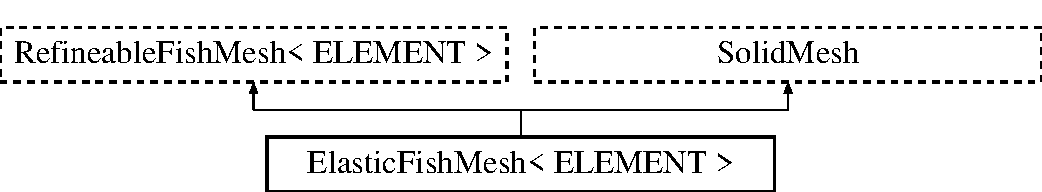
\includegraphics[height=2.000000cm]{classElasticFishMesh}
\end{center}
\end{figure}
\subsection*{Public Member Functions}
\begin{DoxyCompactItemize}
\item 
\hyperlink{classElasticFishMesh_a76c4d63d48b9ee48c3742e55057cfba0}{Elastic\+Fish\+Mesh} (Geom\+Object $\ast$back\+\_\+pt, Geom\+Object $\ast$undeformed\+\_\+back\+\_\+pt, Time\+Stepper $\ast$time\+\_\+stepper\+\_\+pt=\&Mesh\+::\+Default\+\_\+\+Time\+Stepper)
\begin{DoxyCompactList}\small\item\em Constructor\+: Build underlying adaptive fish mesh and then set current Eulerian coordinates to be the Lagrangian ones. Pass pointer to geometric objects that specify the fish\textquotesingle{}s back in the \char`\"{}current\char`\"{} and \char`\"{}undeformed\char`\"{} configurations, and pointer to timestepper (defaults to Static) \end{DoxyCompactList}\item 
virtual \hyperlink{classElasticFishMesh_ab8e084bb7551b9765b95dc38e82ab1be}{$\sim$\+Elastic\+Fish\+Mesh} ()
\begin{DoxyCompactList}\small\item\em Destructor\+: Kill \char`\"{}undeformed\char`\"{} Domain. \end{DoxyCompactList}\end{DoxyCompactItemize}
\subsection*{Private Attributes}
\begin{DoxyCompactItemize}
\item 
Domain $\ast$ \hyperlink{classElasticFishMesh_aef83429a56e87c7218275c1da6c57087}{Undeformed\+\_\+domain\+\_\+pt}
\end{DoxyCompactItemize}


\subsection{Detailed Description}
\subsubsection*{template$<$class E\+L\+E\+M\+E\+NT$>$\newline
class Elastic\+Fish\+Mesh$<$ E\+L\+E\+M\+E\+N\+T $>$}

Refineable fish mesh upgraded to become a solid mesh. 

Definition at line 57 of file static\+\_\+fish.\+cc.



\subsection{Constructor \& Destructor Documentation}
\mbox{\Hypertarget{classElasticFishMesh_a76c4d63d48b9ee48c3742e55057cfba0}\label{classElasticFishMesh_a76c4d63d48b9ee48c3742e55057cfba0}} 
\index{Elastic\+Fish\+Mesh@{Elastic\+Fish\+Mesh}!Elastic\+Fish\+Mesh@{Elastic\+Fish\+Mesh}}
\index{Elastic\+Fish\+Mesh@{Elastic\+Fish\+Mesh}!Elastic\+Fish\+Mesh@{Elastic\+Fish\+Mesh}}
\subsubsection{\texorpdfstring{Elastic\+Fish\+Mesh()}{ElasticFishMesh()}}
{\footnotesize\ttfamily template$<$class E\+L\+E\+M\+E\+NT$>$ \\
\hyperlink{classElasticFishMesh}{Elastic\+Fish\+Mesh}$<$ E\+L\+E\+M\+E\+NT $>$\+::\hyperlink{classElasticFishMesh}{Elastic\+Fish\+Mesh} (\begin{DoxyParamCaption}\item[{Geom\+Object $\ast$}]{back\+\_\+pt,  }\item[{Geom\+Object $\ast$}]{undeformed\+\_\+back\+\_\+pt,  }\item[{Time\+Stepper $\ast$}]{time\+\_\+stepper\+\_\+pt = {\ttfamily \&Mesh\+:\+:Default\+\_\+TimeStepper} }\end{DoxyParamCaption})\hspace{0.3cm}{\ttfamily [inline]}}



Constructor\+: Build underlying adaptive fish mesh and then set current Eulerian coordinates to be the Lagrangian ones. Pass pointer to geometric objects that specify the fish\textquotesingle{}s back in the \char`\"{}current\char`\"{} and \char`\"{}undeformed\char`\"{} configurations, and pointer to timestepper (defaults to Static) 



Definition at line 72 of file static\+\_\+fish.\+cc.

\mbox{\Hypertarget{classElasticFishMesh_ab8e084bb7551b9765b95dc38e82ab1be}\label{classElasticFishMesh_ab8e084bb7551b9765b95dc38e82ab1be}} 
\index{Elastic\+Fish\+Mesh@{Elastic\+Fish\+Mesh}!````~Elastic\+Fish\+Mesh@{$\sim$\+Elastic\+Fish\+Mesh}}
\index{````~Elastic\+Fish\+Mesh@{$\sim$\+Elastic\+Fish\+Mesh}!Elastic\+Fish\+Mesh@{Elastic\+Fish\+Mesh}}
\subsubsection{\texorpdfstring{$\sim$\+Elastic\+Fish\+Mesh()}{~ElasticFishMesh()}}
{\footnotesize\ttfamily template$<$class E\+L\+E\+M\+E\+NT$>$ \\
virtual \hyperlink{classElasticFishMesh}{Elastic\+Fish\+Mesh}$<$ E\+L\+E\+M\+E\+NT $>$\+::$\sim$\hyperlink{classElasticFishMesh}{Elastic\+Fish\+Mesh} (\begin{DoxyParamCaption}{ }\end{DoxyParamCaption})\hspace{0.3cm}{\ttfamily [inline]}, {\ttfamily [virtual]}}



Destructor\+: Kill \char`\"{}undeformed\char`\"{} Domain. 



Definition at line 115 of file static\+\_\+fish.\+cc.



\subsection{Member Data Documentation}
\mbox{\Hypertarget{classElasticFishMesh_aef83429a56e87c7218275c1da6c57087}\label{classElasticFishMesh_aef83429a56e87c7218275c1da6c57087}} 
\index{Elastic\+Fish\+Mesh@{Elastic\+Fish\+Mesh}!Undeformed\+\_\+domain\+\_\+pt@{Undeformed\+\_\+domain\+\_\+pt}}
\index{Undeformed\+\_\+domain\+\_\+pt@{Undeformed\+\_\+domain\+\_\+pt}!Elastic\+Fish\+Mesh@{Elastic\+Fish\+Mesh}}
\subsubsection{\texorpdfstring{Undeformed\+\_\+domain\+\_\+pt}{Undeformed\_domain\_pt}}
{\footnotesize\ttfamily template$<$class E\+L\+E\+M\+E\+NT$>$ \\
Domain$\ast$ \hyperlink{classElasticFishMesh}{Elastic\+Fish\+Mesh}$<$ E\+L\+E\+M\+E\+NT $>$\+::Undeformed\+\_\+domain\+\_\+pt\hspace{0.3cm}{\ttfamily [private]}}

Pointer to \char`\"{}undeformed\char`\"{} Domain -- used to determine the Lagrangian coordinates of any newly created Solid\+Nodes during Mesh refinement 

Definition at line 126 of file static\+\_\+fish.\+cc.



The documentation for this class was generated from the following file\+:\begin{DoxyCompactItemize}
\item 
\hyperlink{static__fish_8cc}{static\+\_\+fish.\+cc}\end{DoxyCompactItemize}

\hypertarget{classElasticFishProblem}{}\section{Elastic\+Fish\+Problem$<$ E\+L\+E\+M\+E\+NT $>$ Class Template Reference}
\label{classElasticFishProblem}\index{Elastic\+Fish\+Problem$<$ E\+L\+E\+M\+E\+N\+T $>$@{Elastic\+Fish\+Problem$<$ E\+L\+E\+M\+E\+N\+T $>$}}


Boundary-\/driven elastic deformation of fish-\/shaped domain.  


Inheritance diagram for Elastic\+Fish\+Problem$<$ E\+L\+E\+M\+E\+NT $>$\+:\begin{figure}[H]
\begin{center}
\leavevmode
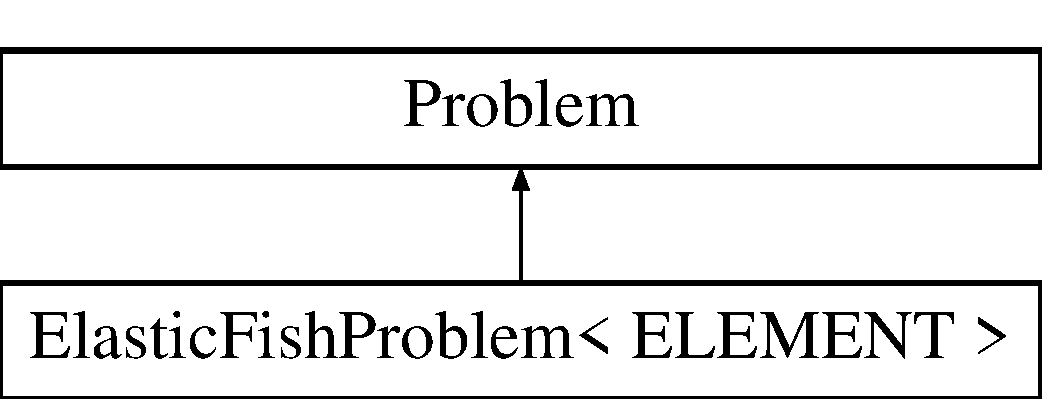
\includegraphics[height=2.000000cm]{classElasticFishProblem}
\end{center}
\end{figure}
\subsection*{Public Member Functions}
\begin{DoxyCompactItemize}
\item 
\hyperlink{classElasticFishProblem_adf9fdb0b94ac76b7fdb34bc7fa809a41}{Elastic\+Fish\+Problem} ()
\begin{DoxyCompactList}\small\item\em Constructor\+: \end{DoxyCompactList}\item 
void \hyperlink{classElasticFishProblem_aaaf23036d8f282cff88e497ad214237f}{run} ()
\begin{DoxyCompactList}\small\item\em Run simulation. \end{DoxyCompactList}\item 
\hyperlink{classElasticFishMesh}{Elastic\+Fish\+Mesh}$<$ E\+L\+E\+M\+E\+NT $>$ $\ast$ \hyperlink{classElasticFishProblem_a616c07228c52c594f90dfb1333015712}{mesh\+\_\+pt} ()
\begin{DoxyCompactList}\small\item\em Access function for the mesh. \end{DoxyCompactList}\item 
void \hyperlink{classElasticFishProblem_a5cd7dbd2bc99ccf850c1a58d0b401979}{doc\+\_\+solution} (Doc\+Info \&doc\+\_\+info)
\begin{DoxyCompactList}\small\item\em Doc the solution. \end{DoxyCompactList}\item 
void \hyperlink{classElasticFishProblem_a41badf8aa60bf52d888338039168fcb3}{actions\+\_\+after\+\_\+newton\+\_\+solve} ()
\begin{DoxyCompactList}\small\item\em Update function (empty) \end{DoxyCompactList}\item 
void \hyperlink{classElasticFishProblem_a7c22fcff8d94166797e87d70017540d6}{actions\+\_\+before\+\_\+newton\+\_\+solve} ()
\begin{DoxyCompactList}\small\item\em Update before solve\+: We\textquotesingle{}re dealing with a static problem so the nodal positions before the next solve merely serve as initial conditions. For meshes that are very strongly refined near the boundary, the update of the displacement boundary conditions (which only moves the Solid\+Nodes {\itshape on} the boundary), can lead to strongly distorted meshes. This can cause the Newton method to fail --$>$ the overall method is actually more robust if we use the nodal positions as determined by the Domain/\+Macro\+Element-\/ based mesh update as initial guesses. \end{DoxyCompactList}\item 
void \hyperlink{classElasticFishProblem_ae54b974caafe717309ce7abc5e7f824d}{actions\+\_\+after\+\_\+adapt} ()
\begin{DoxyCompactList}\small\item\em Update after adapt\+: Pin all redundant pressure nodes (if required) \end{DoxyCompactList}\end{DoxyCompactItemize}
\subsection*{Private Attributes}
\begin{DoxyCompactItemize}
\item 
Circle $\ast$ \hyperlink{classElasticFishProblem_a1a026c063e41c004f656988d6bfd541b}{Fish\+\_\+back\+\_\+pt}
\end{DoxyCompactItemize}


\subsection{Detailed Description}
\subsubsection*{template$<$class E\+L\+E\+M\+E\+NT$>$\newline
class Elastic\+Fish\+Problem$<$ E\+L\+E\+M\+E\+N\+T $>$}

Boundary-\/driven elastic deformation of fish-\/shaped domain. 

Definition at line 185 of file static\+\_\+fish.\+cc.



\subsection{Constructor \& Destructor Documentation}
\mbox{\Hypertarget{classElasticFishProblem_adf9fdb0b94ac76b7fdb34bc7fa809a41}\label{classElasticFishProblem_adf9fdb0b94ac76b7fdb34bc7fa809a41}} 
\index{Elastic\+Fish\+Problem@{Elastic\+Fish\+Problem}!Elastic\+Fish\+Problem@{Elastic\+Fish\+Problem}}
\index{Elastic\+Fish\+Problem@{Elastic\+Fish\+Problem}!Elastic\+Fish\+Problem@{Elastic\+Fish\+Problem}}
\subsubsection{\texorpdfstring{Elastic\+Fish\+Problem()}{ElasticFishProblem()}}
{\footnotesize\ttfamily template$<$class E\+L\+E\+M\+E\+NT $>$ \\
\hyperlink{classElasticFishProblem}{Elastic\+Fish\+Problem}$<$ E\+L\+E\+M\+E\+NT $>$\+::\hyperlink{classElasticFishProblem}{Elastic\+Fish\+Problem} (\begin{DoxyParamCaption}{ }\end{DoxyParamCaption})}



Constructor\+: 



Definition at line 241 of file static\+\_\+fish.\+cc.



References Global\+\_\+\+Physical\+\_\+\+Variables\+::body\+\_\+force(), and Global\+\_\+\+Physical\+\_\+\+Variables\+::\+Constitutive\+\_\+law\+\_\+pt.



\subsection{Member Function Documentation}
\mbox{\Hypertarget{classElasticFishProblem_ae54b974caafe717309ce7abc5e7f824d}\label{classElasticFishProblem_ae54b974caafe717309ce7abc5e7f824d}} 
\index{Elastic\+Fish\+Problem@{Elastic\+Fish\+Problem}!actions\+\_\+after\+\_\+adapt@{actions\+\_\+after\+\_\+adapt}}
\index{actions\+\_\+after\+\_\+adapt@{actions\+\_\+after\+\_\+adapt}!Elastic\+Fish\+Problem@{Elastic\+Fish\+Problem}}
\subsubsection{\texorpdfstring{actions\+\_\+after\+\_\+adapt()}{actions\_after\_adapt()}}
{\footnotesize\ttfamily template$<$class E\+L\+E\+M\+E\+NT$>$ \\
void \hyperlink{classElasticFishProblem}{Elastic\+Fish\+Problem}$<$ E\+L\+E\+M\+E\+NT $>$\+::actions\+\_\+after\+\_\+adapt (\begin{DoxyParamCaption}{ }\end{DoxyParamCaption})\hspace{0.3cm}{\ttfamily [inline]}}



Update after adapt\+: Pin all redundant pressure nodes (if required) 



Definition at line 222 of file static\+\_\+fish.\+cc.

\mbox{\Hypertarget{classElasticFishProblem_a41badf8aa60bf52d888338039168fcb3}\label{classElasticFishProblem_a41badf8aa60bf52d888338039168fcb3}} 
\index{Elastic\+Fish\+Problem@{Elastic\+Fish\+Problem}!actions\+\_\+after\+\_\+newton\+\_\+solve@{actions\+\_\+after\+\_\+newton\+\_\+solve}}
\index{actions\+\_\+after\+\_\+newton\+\_\+solve@{actions\+\_\+after\+\_\+newton\+\_\+solve}!Elastic\+Fish\+Problem@{Elastic\+Fish\+Problem}}
\subsubsection{\texorpdfstring{actions\+\_\+after\+\_\+newton\+\_\+solve()}{actions\_after\_newton\_solve()}}
{\footnotesize\ttfamily template$<$class E\+L\+E\+M\+E\+NT$>$ \\
void \hyperlink{classElasticFishProblem}{Elastic\+Fish\+Problem}$<$ E\+L\+E\+M\+E\+NT $>$\+::actions\+\_\+after\+\_\+newton\+\_\+solve (\begin{DoxyParamCaption}{ }\end{DoxyParamCaption})\hspace{0.3cm}{\ttfamily [inline]}}



Update function (empty) 



Definition at line 204 of file static\+\_\+fish.\+cc.

\mbox{\Hypertarget{classElasticFishProblem_a7c22fcff8d94166797e87d70017540d6}\label{classElasticFishProblem_a7c22fcff8d94166797e87d70017540d6}} 
\index{Elastic\+Fish\+Problem@{Elastic\+Fish\+Problem}!actions\+\_\+before\+\_\+newton\+\_\+solve@{actions\+\_\+before\+\_\+newton\+\_\+solve}}
\index{actions\+\_\+before\+\_\+newton\+\_\+solve@{actions\+\_\+before\+\_\+newton\+\_\+solve}!Elastic\+Fish\+Problem@{Elastic\+Fish\+Problem}}
\subsubsection{\texorpdfstring{actions\+\_\+before\+\_\+newton\+\_\+solve()}{actions\_before\_newton\_solve()}}
{\footnotesize\ttfamily template$<$class E\+L\+E\+M\+E\+NT$>$ \\
void \hyperlink{classElasticFishProblem}{Elastic\+Fish\+Problem}$<$ E\+L\+E\+M\+E\+NT $>$\+::actions\+\_\+before\+\_\+newton\+\_\+solve (\begin{DoxyParamCaption}{ }\end{DoxyParamCaption})\hspace{0.3cm}{\ttfamily [inline]}}



Update before solve\+: We\textquotesingle{}re dealing with a static problem so the nodal positions before the next solve merely serve as initial conditions. For meshes that are very strongly refined near the boundary, the update of the displacement boundary conditions (which only moves the Solid\+Nodes {\itshape on} the boundary), can lead to strongly distorted meshes. This can cause the Newton method to fail --$>$ the overall method is actually more robust if we use the nodal positions as determined by the Domain/\+Macro\+Element-\/ based mesh update as initial guesses. 



Definition at line 215 of file static\+\_\+fish.\+cc.

\mbox{\Hypertarget{classElasticFishProblem_a5cd7dbd2bc99ccf850c1a58d0b401979}\label{classElasticFishProblem_a5cd7dbd2bc99ccf850c1a58d0b401979}} 
\index{Elastic\+Fish\+Problem@{Elastic\+Fish\+Problem}!doc\+\_\+solution@{doc\+\_\+solution}}
\index{doc\+\_\+solution@{doc\+\_\+solution}!Elastic\+Fish\+Problem@{Elastic\+Fish\+Problem}}
\subsubsection{\texorpdfstring{doc\+\_\+solution()}{doc\_solution()}}
{\footnotesize\ttfamily template$<$class E\+L\+E\+M\+E\+NT $>$ \\
void \hyperlink{classElasticFishProblem}{Elastic\+Fish\+Problem}$<$ E\+L\+E\+M\+E\+NT $>$\+::doc\+\_\+solution (\begin{DoxyParamCaption}\item[{Doc\+Info \&}]{doc\+\_\+info }\end{DoxyParamCaption})}



Doc the solution. 



Definition at line 331 of file static\+\_\+fish.\+cc.

\mbox{\Hypertarget{classElasticFishProblem_a616c07228c52c594f90dfb1333015712}\label{classElasticFishProblem_a616c07228c52c594f90dfb1333015712}} 
\index{Elastic\+Fish\+Problem@{Elastic\+Fish\+Problem}!mesh\+\_\+pt@{mesh\+\_\+pt}}
\index{mesh\+\_\+pt@{mesh\+\_\+pt}!Elastic\+Fish\+Problem@{Elastic\+Fish\+Problem}}
\subsubsection{\texorpdfstring{mesh\+\_\+pt()}{mesh\_pt()}}
{\footnotesize\ttfamily template$<$class E\+L\+E\+M\+E\+NT$>$ \\
\hyperlink{classElasticFishMesh}{Elastic\+Fish\+Mesh}$<$E\+L\+E\+M\+E\+NT$>$$\ast$ \hyperlink{classElasticFishProblem}{Elastic\+Fish\+Problem}$<$ E\+L\+E\+M\+E\+NT $>$\+::mesh\+\_\+pt (\begin{DoxyParamCaption}{ }\end{DoxyParamCaption})\hspace{0.3cm}{\ttfamily [inline]}}



Access function for the mesh. 



Definition at line 197 of file static\+\_\+fish.\+cc.

\mbox{\Hypertarget{classElasticFishProblem_aaaf23036d8f282cff88e497ad214237f}\label{classElasticFishProblem_aaaf23036d8f282cff88e497ad214237f}} 
\index{Elastic\+Fish\+Problem@{Elastic\+Fish\+Problem}!run@{run}}
\index{run@{run}!Elastic\+Fish\+Problem@{Elastic\+Fish\+Problem}}
\subsubsection{\texorpdfstring{run()}{run()}}
{\footnotesize\ttfamily template$<$class E\+L\+E\+M\+E\+NT $>$ \\
void \hyperlink{classElasticFishProblem}{Elastic\+Fish\+Problem}$<$ E\+L\+E\+M\+E\+NT $>$\+::run (\begin{DoxyParamCaption}{ }\end{DoxyParamCaption})}



Run simulation. 

Run the problem. 

Definition at line 358 of file static\+\_\+fish.\+cc.



References Global\+\_\+\+Physical\+\_\+\+Variables\+::\+Gravity.



Referenced by main().



\subsection{Member Data Documentation}
\mbox{\Hypertarget{classElasticFishProblem_a1a026c063e41c004f656988d6bfd541b}\label{classElasticFishProblem_a1a026c063e41c004f656988d6bfd541b}} 
\index{Elastic\+Fish\+Problem@{Elastic\+Fish\+Problem}!Fish\+\_\+back\+\_\+pt@{Fish\+\_\+back\+\_\+pt}}
\index{Fish\+\_\+back\+\_\+pt@{Fish\+\_\+back\+\_\+pt}!Elastic\+Fish\+Problem@{Elastic\+Fish\+Problem}}
\subsubsection{\texorpdfstring{Fish\+\_\+back\+\_\+pt}{Fish\_back\_pt}}
{\footnotesize\ttfamily template$<$class E\+L\+E\+M\+E\+NT$>$ \\
Circle$\ast$ \hyperlink{classElasticFishProblem}{Elastic\+Fish\+Problem}$<$ E\+L\+E\+M\+E\+NT $>$\+::Fish\+\_\+back\+\_\+pt\hspace{0.3cm}{\ttfamily [private]}}



Definition at line 233 of file static\+\_\+fish.\+cc.



The documentation for this class was generated from the following file\+:\begin{DoxyCompactItemize}
\item 
\hyperlink{static__fish_8cc}{static\+\_\+fish.\+cc}\end{DoxyCompactItemize}

\chapter{File Documentation}
\hypertarget{static__fish_8cc}{}\section{static\+\_\+fish.\+cc File Reference}
\label{static__fish_8cc}\index{static\+\_\+fish.\+cc@{static\+\_\+fish.\+cc}}
\subsection*{Classes}
\begin{DoxyCompactItemize}
\item 
class \hyperlink{classElasticFishMesh}{Elastic\+Fish\+Mesh$<$ E\+L\+E\+M\+E\+N\+T $>$}
\begin{DoxyCompactList}\small\item\em Refineable fish mesh upgraded to become a solid mesh. \end{DoxyCompactList}\item 
class \hyperlink{classElasticFishProblem}{Elastic\+Fish\+Problem$<$ E\+L\+E\+M\+E\+N\+T $>$}
\begin{DoxyCompactList}\small\item\em Boundary-\/driven elastic deformation of fish-\/shaped domain. \end{DoxyCompactList}\end{DoxyCompactItemize}
\subsection*{Namespaces}
\begin{DoxyCompactItemize}
\item 
 \hyperlink{namespaceGlobal__Physical__Variables}{Global\+\_\+\+Physical\+\_\+\+Variables}
\begin{DoxyCompactList}\small\item\em Global variables. \end{DoxyCompactList}\end{DoxyCompactItemize}
\subsection*{Functions}
\begin{DoxyCompactItemize}
\item 
void \hyperlink{namespaceGlobal__Physical__Variables_a313e702a9e8fdec808702c9bbf38b192}{Global\+\_\+\+Physical\+\_\+\+Variables\+::body\+\_\+force} (const double \&t, const Vector$<$ double $>$ \&xi, Vector$<$ double $>$ \&b)
\begin{DoxyCompactList}\small\item\em Body force vector\+: Vertically downwards with magnitude Gravity. \end{DoxyCompactList}\item 
int \hyperlink{static__fish_8cc_ae66f6b31b5ad750f1fe042a706a4e3d4}{main} ()
\begin{DoxyCompactList}\small\item\em Driver for simple elastic problem. \end{DoxyCompactList}\end{DoxyCompactItemize}
\subsection*{Variables}
\begin{DoxyCompactItemize}
\item 
Strain\+Energy\+Function $\ast$ \hyperlink{namespaceGlobal__Physical__Variables_a73135f793690b4386bf83bbefc7bf310}{Global\+\_\+\+Physical\+\_\+\+Variables\+::\+Strain\+\_\+energy\+\_\+function\+\_\+pt}
\begin{DoxyCompactList}\small\item\em Pointer to strain energy function. \end{DoxyCompactList}\item 
Constitutive\+Law $\ast$ \hyperlink{namespaceGlobal__Physical__Variables_a2a37fb040c832ee7a086bb13bb02a100}{Global\+\_\+\+Physical\+\_\+\+Variables\+::\+Constitutive\+\_\+law\+\_\+pt}
\begin{DoxyCompactList}\small\item\em Pointer to constitutive law. \end{DoxyCompactList}\item 
double \hyperlink{namespaceGlobal__Physical__Variables_a09a019474b7405b35da2437f7779bc7e}{Global\+\_\+\+Physical\+\_\+\+Variables\+::E} =1.\+0
\begin{DoxyCompactList}\small\item\em Elastic modulus. \end{DoxyCompactList}\item 
double \hyperlink{namespaceGlobal__Physical__Variables_a3962c36313826b19f216f6bbbdd6a477}{Global\+\_\+\+Physical\+\_\+\+Variables\+::\+Nu} =0.\+3
\begin{DoxyCompactList}\small\item\em Poisson\textquotesingle{}s ratio. \end{DoxyCompactList}\item 
double \hyperlink{namespaceGlobal__Physical__Variables_a849754fa7155c1a31481674ce4845658}{Global\+\_\+\+Physical\+\_\+\+Variables\+::\+C1} =1.\+3
\begin{DoxyCompactList}\small\item\em \char`\"{}\+Mooney Rivlin\char`\"{} coefficient for generalised Mooney Rivlin law \end{DoxyCompactList}\item 
double \hyperlink{namespaceGlobal__Physical__Variables_a8b80d3e8d63b8d0a0ed435a2dd7fe2ad}{Global\+\_\+\+Physical\+\_\+\+Variables\+::\+Gravity} =0.\+0
\begin{DoxyCompactList}\small\item\em Body force. \end{DoxyCompactList}\end{DoxyCompactItemize}


\subsection{Function Documentation}
\mbox{\Hypertarget{static__fish_8cc_ae66f6b31b5ad750f1fe042a706a4e3d4}\label{static__fish_8cc_ae66f6b31b5ad750f1fe042a706a4e3d4}} 
\index{static\+\_\+fish.\+cc@{static\+\_\+fish.\+cc}!main@{main}}
\index{main@{main}!static\+\_\+fish.\+cc@{static\+\_\+fish.\+cc}}
\subsubsection{\texorpdfstring{main()}{main()}}
{\footnotesize\ttfamily int main (\begin{DoxyParamCaption}{ }\end{DoxyParamCaption})}



Driver for simple elastic problem. 



Definition at line 396 of file static\+\_\+fish.\+cc.



References Global\+\_\+\+Physical\+\_\+\+Variables\+::\+C1, Global\+\_\+\+Physical\+\_\+\+Variables\+::\+Constitutive\+\_\+law\+\_\+pt, Global\+\_\+\+Physical\+\_\+\+Variables\+::E, Global\+\_\+\+Physical\+\_\+\+Variables\+::\+Nu, Elastic\+Fish\+Problem$<$ E\+L\+E\+M\+E\+N\+T $>$\+::run(), and Global\+\_\+\+Physical\+\_\+\+Variables\+::\+Strain\+\_\+energy\+\_\+function\+\_\+pt.


\hypertarget{static__fish_8txt__doxygenified_8h}{}\section{static\+\_\+fish.\+txt\+\_\+doxygenified.\+h File Reference}
\label{static__fish_8txt__doxygenified_8h}\index{static\+\_\+fish.\+txt\+\_\+doxygenified.\+h@{static\+\_\+fish.\+txt\+\_\+doxygenified.\+h}}

%--- End generated contents ---

% Index
\backmatter
\newpage
\phantomsection
\clearemptydoublepage
\addcontentsline{toc}{chapter}{Index}
\printindex

